\section{Starting Well}
% Need to go through with Verity and discuss the hot button issues that can be covered in this section
\subsection{Summary}
{\bfseries The early years of life lay foundations for lifelong physical, emotional and mental health, wellbeing and resilience. In tackling inequalities, action taken in the early years of life can have lifelong benefit, with many interventions being highly cost-effective.

There are 193,200 children and young people aged 0-19 years in West Sussex, with approximately 8,000 births a year. Across the county overall, 22\% of the population are 0-19 years, which is lower compared with England (24\%). Within the county, Crawley has a much younger population, with 26\% of residents aged 0-19 years.}

Overall measures of infant and maternal health in West Sussex are good, but inequalities are apparent across the county and in relation to specific groups. 
\begin{itemize}
    \item The infant mortality rate remains below the national rate (3.6 per 1,000 live births compared with 3.9 nationally)\footnote{PHOF E01, 2018-2020.}, we have fewer low birth weight babies, a lower percentage of women who smoke at the time of delivery, and a higher proportion of children who are assessed as having a good level of development at their two year check. 
\end{itemize}

However there remain challenges in the early years of life. 

\begin{itemize}[noitemsep]
    \item Many immunisation rates, whilst higher than national levels, remain below target levels.
    \item Measures relating to child readiness for school have improved in recent years but remain lower than many comparable authorities and for children eligible for a free school meal. For example, in 2018/19, approximately 72\% of children achieved a good level of development at the end of Reception whilst only 51\% were assessed as having a good level of development, the third lowest of comparable authorities.
\end{itemize}

We continue to observe a strong social gradient across many indicators and outcomes. Children living in poverty and from deprived areas are more likely to be overweight or obese; less likely to attain the expected level of attainment across educational key stages; more likely to admitted to hospital for self-harm; more likely to become pregnant as a teenager; and more likely to grow up in a household where someone smokes. 

In West Sussex, almost 17,000 children live in poverty. Children in poverty are more likely to come from single parent/carer families, be disabled or live in a household with an adult who is disabled. Poverty can transmit across generations and there are specific concerns about low social mobility in some parts of the county. 

It is also important to recognise that, on average, children who are in care or are care leavers have significantly poorer health and educational outcomes than their peers. 

Emotional and mental health are instrinically linked to physical wellbeing and longer term outcomes. Children who are happier and more emotionally resilient tend to have better physical health. Local survey data has highlighted the importance of cognitive reappriasal (reframing problems in a positive way) and expressive suppression (burying negative feelings/avoidance) in predicting life satisfaction and overall happiness\footnote{For more details, please see the 2019/20 JSNA Strategy.}.

% Children in low income families can be found on Stat-x-plore https://stat-xplore.dwp.gov.uk/webapi/jsf/dataCatalogueExplorer.xhtml

% \subsection{Impact of Covid-19 Pandemic}
% \todo[inline]{Use the WICH tool to support this part of the narrative. Some of the indicators involve children and young people. November 2021 access.}

\subsection{Infant and Maternal Health}
Key demographic information and health indicators are summarised in the West Sussex Local Health Profiles for Children and Young People 2020, available on the JSNA website.

\subsubsection{Infant and Maternal Health}
{\bfseries In 2020 there were 8,001 births,} the lowest number in West Sussex since 2006. The infant mortality rate\footnote{PHOF reference E01, defined as the number of deaths in infants aged under 1 year per 1,000 live births.} in 2018-2020 was 3.6 per 1,000 live births, lower than the national rate of 3.9 per 1,000, although a slight increase on the previous three years.

The {\bfseries neonatal mortality rate} (defined as the number of deaths under 28 days, per 1,000 live births) has remained stable over the past 10 years, although there has been a slight rise in both 2017-2019 and 2018-2020. The rate in West Sussex 3.6 per 1,000 live births, in line with the England rate (3.9 per 1,000) and below the median of the south east region. 

{\bfseries The percentage of term babies with low birth weight (less than 2500g; \footnote{PHOF reference C04.}) remains steady}, at 2.04\% in 2020, and significantly lower than England (2.9\%) and in the lowest three of CIPFA neighbours.

In 2018-20, there were {\bfseries 78.6 premature births (less than 37 weeks gestation) per 1,000} live births and still births, which is the lowest it has been since 2011-13 (76.6 per 1,000). The rate in West Sussex has followed national trends, and is in line with the England rate of 79.1 per 1,000.

The multiple birth rate (the number of maternities with multiple births per 1,000 total maternities) in 2020 was 11.0 ({\bfseries 87 multiple births}), lower than the England rate of 14.4.

{\bfseries In 2020/21, 34.1\% of births were by caesarean section in West Sussex.} This proportion has been increasing over the last 5 years and is significantly higher compared to England (32.5\%) and is also the second highest among five comparable authorities\footnote{NOTE: these comparable authorities are not the standard CIPFA neighbours, but rather the Children's Services Statistical Neighbours as provided by LAIT.}.

{\bfseries The percentage of women smoking at the time of delivery\footnote{PHOF reference C06. Note: the method used to calculate this outcome was changed in April 2017, excluding women with unknown smoking status from the denominator when calculating the proportion of women smoking at the time of delivery.} remained low in 2020/21 at 8.5\% (approximately 678 maternities)}, lower than the national rate and the second lowest of comparable authorities.

In 2019/20, 55.7\% of women breastfed (wholly or partly) at 6-8 weeks\footnote{PHOF reference C05b.}. Nationally, the figure was 48\%. West Sussex was the second highest of comparable authorities. Note that this indicator is not available for 2020/21 due to data quality issues.

In 2020/21, 91.5\% of New Birth Visits (NBVs)\footnote{PHOF reference C07. All infants and their families are eligible to receive a visit led by a health visitor within the first two weeks from birth, as part of the Healthy Child Programme and to ensure continuing support following midwife visits, which usually end at day 10. For 2020/21, this indicator was scaled up from three quarters worth of available data.} were completed within 14 days this has increased to be above the England rate (88.0\%).

In 2020/21, 84\% of children assessed achieved a good level of development at 2-2½ years\footnote{PHOF reference C08a. For 2020/21, this indicator was scaled up from three quarters worth of available data.}, comparing well with England (82.9\%), and making West Sussex the fifth highest amongst comparable local authorities.

Uptake of the flu vaccine in 2-3 year-olds\footnote{PHOF reference D03l.} in 2020/21 was 67.5\% and was significantly higher than England (56.7\%) and the $\geq$65\% benchmark.

% \todo[inline]{check MEASLES}In 2018, there were 45 laboratory confirmed cases of measles in West Sussex, representing a rate of 5.3 per 100,000 population, the highest amongst comparable authorities and the 16th highest in England.

\subsubsection{Maternal Mental Health} In relation to maternal mental health, it is estimated that between 10\% and 20\% of women will be affected by mental health problems, either during their pregnancy or in the first year post delivery. Local data are scarce but using synthetic estimates provided by Public Health England, the number of mothers with specific problems are shown below (note some women will be affected by one or more problems):
\begin{itemize}[noitemsep]
    \item Postpartum psychosis: 20 
    \item Chronic Severe Mental Illness: 20
    \item Severe depressive illness: 250 
    \item Mild-moderate depressive illness and anxiety: 830 (lower estimate) to 1,245 (upper estimate) 
    \item PTSD: 250 
    \item Adjustment disorders and distress: 1,245 (lower estimate) to 2,485 (upper estimate)
\end{itemize}

\subsection{West Sussex Childhood Vaccine and Immunisation Coverage Rates}
See Table~\ref{tab:childhoodimms} on page~\pageref{tab:childhoodimms}.
\begin{table*}[hbt]
    \scriptsize
    \caption{West Sussex Childhood Vaccine and Immunisation Coverage Rates. PHOF references (all, except Hib/Men C booster in under-5s are PHOF indicators) D03b to D03f; D03h to D03m; D04a to D04c; D04e; D04f; Cl.2}
    \centering
    \begin{tabular}{llrrrr}
    \toprule
    Immunisation &  Detail & Year & \% Coverage & Lower CI & Upper CI \\
    \midrule
    Rotavirus & \% of children who have received the rotavirus vaccine by 6 months of age & 2019/20	& 91.90\% & 91.40\% & 92.50\% \\
    Hepatitis B & \% of children at age 12 months who have received the complete course (3 doses) of hepatitis B vaccine. & 2019/20	& 100\% & 75.80\% & 100\% \\
    DTaP / IPV / Hib & \% of children who received 3 doses of DTaP/IPV/Hib vaccine at any time by their rst birthday. & 2019/20	& 95.40\% & 94.40\% & 96.50\% \\
    MenB & \% of children who received the MenB vaccine at any time before their rst birthday & 2019/20	& 95.40\% & 94.90\% & 95.80\% \\
    PCV & \% of children who received two doses of PCV at any time before their first birthday. & 2019/20 & 95.80\% & 95.30\% & 96.20\% \\
    MenC & \% of children who received 2 doses of MenC vaccine at any time by their rst birthday. & 2015/16 & 94.3 & 93.8 & 94.7 \\
    Hib / MenC booster & \% of children who received a booster dose of Hib/MenC at any time before 2nd birthday. & 2019/20 & 94.60\% & 94.20\% & 95.10\% \\
    MMR one dose & \% of children who received one dose of MMR on or after their first birthday and at any time before their 2nd birthday. & 2019/20 & 94.70\% & 94.30\% & 95.20\% \\
    Hepatitis B & \% of children at age 24 months who have received the complete course (4 doses) of hepatitis B vaccine. & 2019/20 & suppressed & - & - \\
    DTaP / IPV / Hib & \% of children who received 3 doses of DTaP/IPV/Hib at any time before their 2nd birthday & 2018/19 & 95.7 & 95.3 & 96.1 \\
    PCV booster & \% of children who received a booster dose of PCV at any time before their 2nd birthday & 2019/20 & 94.40\% & 93.90\% & 94.90\% \\
    MenB booster & \% of children who received a booster dose of MenB at any time before their 2nd birthday & 2019/20 & 93.20\% & 92.70\% & 93.70\% \\
    Flu & \% children aged 2-3 years old, who received the Flu vaccination (1st Sept to the end of Feb) in a primary care setting & 2019/20 & 53.50\% & 52.80\% & 54.30\% \\
    DTaP / IPV & \% of children who received a booster dose of DTaP/IPV at any time before their fifth birthday & 2019/20 & 89.30\% & 88.60\% & 89.90\% \\
    MMR for one dose & \% of children who received one dose of MMR on or after their first birthday and at any time before their fifth birthday. & 2019/20 & 95.70\% & 95.20\% & 96.00\% \\
    MMR for two doses & \% of children who received two doses of MMR on or after their first birthday and at any time before their fifth birthday. &  2019/20 & 91.60\% & 91.10\% & 92.10\% \\
    Hib / Men C booster & \% of children who received a booster dose of Hib/MenC at any time before their fifth birthday. & 2017/18 & 92.6 & 92.1 & 93.1 \\
    HPV - one dose & \% of females in school year 8 (aged 12-13) who have received the first dose of HPV vaccine & 2019/20 & 14.90\% & 13.90\% & 15.90\% \\
    HPV - two doses & \% of females in school year 8/9 (aged 13-14) who have received the second (completing) dose of HPV vaccine & 2019/20 & 11.30\% &10.40\% & 12.30\% \\
    \bottomrule
\end{tabular}
\label{tab:childhoodimms}
\end{table*}
\normalsize
\subsection{Hospital admissions}
\paragraph{Emergency admissions}In 2020/21, West Sussex had among the highest emergency hospital admission rates in the South East, and rates were higher than national rates:
\begin{itemize}[noitemsep]
    \item {\bfseries Under 1 years old -- 2,500 admissions,} a rate of 253.4 per 1,000 population.
    \item {\bfseries 0-4 year olds -- 4,880 admissions,} a rate of 107.4 per 1,000 population.
    \item {\bfseries Under 18s -- 9,480 admissions,} a rate of 53.4 per 1,000 population.
\end{itemize}
\paragraph{Admissions to hospital - 0-19 year olds}
\begin{itemize}[noitemsep]
    \item {\bfseries Asthma -- 100 admissions (2020/21)}, a rate of 53.8 per 100,000 population, lower than England and comparable authorities.
    \item {\bfseries Diabetes -- 115 admissions (2019/20)}, a rate of 62.2 per 100,000 higher than England and comparable authorities.
    \item {\bfseries Epilepsy -- 125 admissions (2019/20)}, a rate of 67.6 per 100,000, similar to England and comparable authorities.
\end{itemize}

\subsection{Disability through the life course}
\paragraph{Overall Disability Assumption} The term "disability" is frequently used but often poorly defined, and estimating the prevalence and type of disability within a population is difficult. The purpose of a definition (for example, for deciding educational support vs. eligibility for welfare benefits), as opposed to a "formal diagnosis" can mean that different sources can often provide very different pictures of the local population.

The Family Resources Survey (FRS) is a national, continuous household survey that collects data on a wide range of information including disability\footnote{{\bf The definition of "disability" in the Family Resource Survey is} used to describe people who identify themselves or have been identified as having any physical or mental health condition or illness that lasts or is expected to last 12 months or more, and acts to limit the ability to carry out day-to-day activities. While this will capture most people under the definition used in the Equality Act 2010, it should be noted that there will be some people under the 2010 Act who are classified as disabled (and having rights under the Act) who have a long-standing illness or disability which is not currently affecting their day-to-day activities e.g. some people who have a diagnosis of cancer will not be included.}, caring, tenure and income. One of the main functions of the survey is to inform the Department of Work and Pensions (DWP) of the living conditions and economic circumstances of different households. Small sample size means that data are not published below regional level. Using the results from the latest national survey and applying the prevalence to the local population provides a local estimate of disability by age groups. Given that West Sussex overall has a relatively healthy and wealthy population, these estimates may be higher than expected and should be treated as possibly high estimates.

\begin{figure}[htp]
    \caption{Disability by age group and gender}
    \centering
	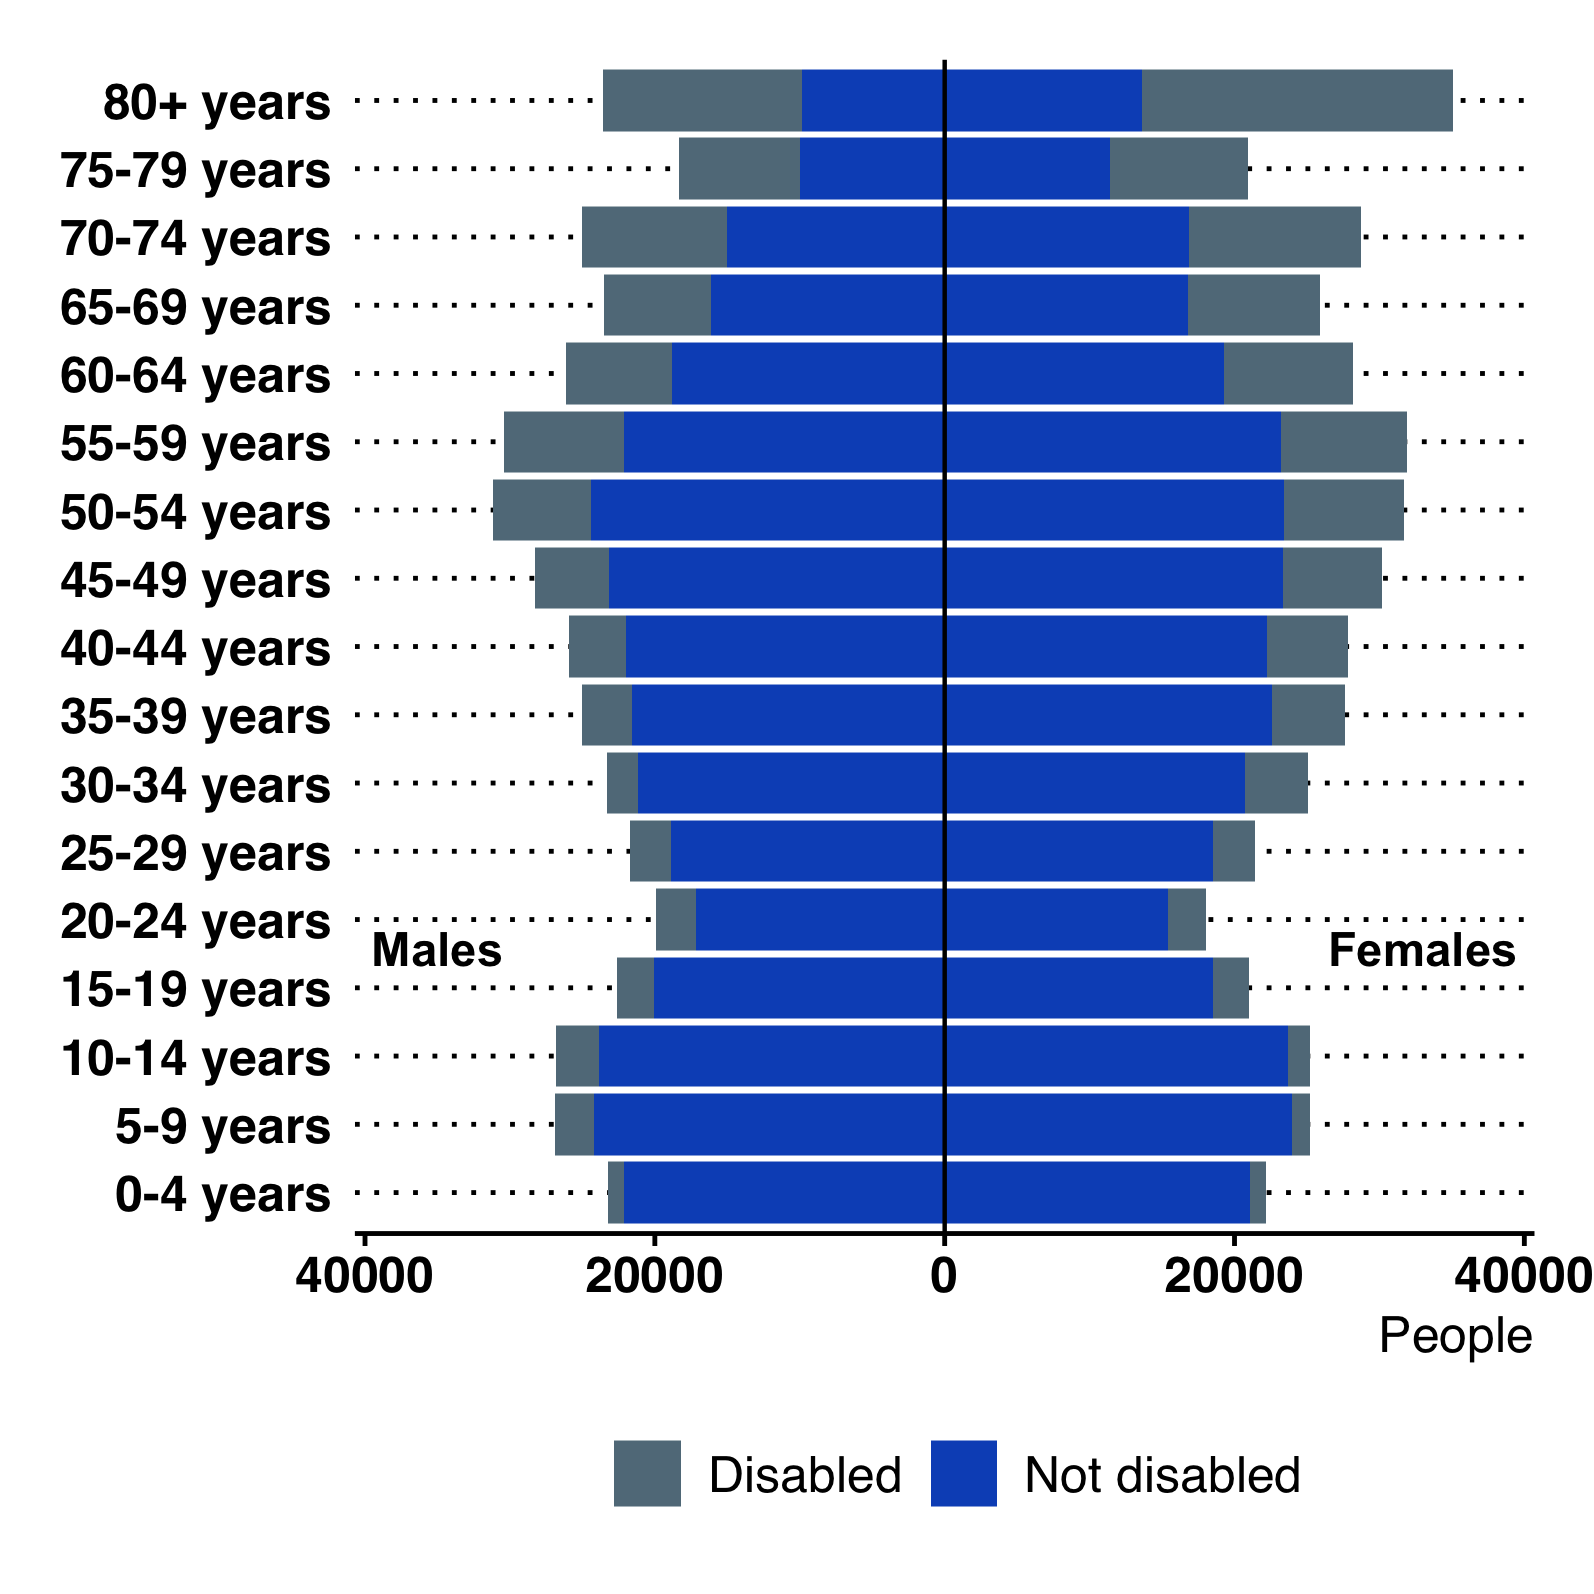
\includegraphics[width=\linewidth]{images/frs_disability_wsx.png}
	\label{fig:frs_diab_wsx}
\end{figure}

FRS Disability Prevalence (average of years 2014/15 to 2017/18) Applied to 2018 West Sussex Population TABLE\todo[inline]{Where did I put this?}

\paragraph{FRS Type of Impairment} Of people who described themselves as being disabled, data were also collected on the nature of their impairment. As people are able to state multiple impairments, figures in Table~\ref{tab:impairment} do not sum 100.

Nationally it is noted that the proportion of FRS respondents who reported a mental health impairment has been rising in recent years, from 22\% in 2015/16 to 25\% in 2017/18.\todo[inline]{Check this}

Note again that, given West Sussex overall has a relatively healthy and wealthy population, these estimates may be higher than expected and should be treated as possibly high estimates.

\begin{table}[hbt]
    \caption{FRS Type of Impairment}
    \centering
    \begin{tabular}{lllll}
    \toprule
    Impairment & All Disabled & Children & Working & State \\
    type (\%) & People & \ & age & Pension \\
    \midrule
    Mobility & 49 & 19 & 41 & 67 \\
    Stamina, breathing \& fatigue & 37 & 24 & 32 & 46 \\
    %and fatigue & \ & \ & \ & \ \\
    Dexterity & 26 & 11 & 23 & 34 \\
    Mental health & 25 & 23 & 38 & 9 \\
    Memory & 16 & 11 & 16 & 17 \\
    Hearing & 14 & 8 & 8 & 23 \\
    Vision & 12 & 9 & 9 & 18 \\
    Learning & 13 & 36 & 14 & 8 \\
    Social/behavioural & 9 & 43 & 10 & 2 \\
    Other & 17 & 18 & 18 & 15 \\
    \bottomrule
    \end{tabular}
    \label{tab:impairment}
\end{table}

\subsection{Mental Health and Wellbeing}
{\bfseries Major national surveys remain the best source of evidence on the prevalence of mental health disorders among children and young people.}

In 2004, ONS conducted a national survey to estimate the prevalence of mental health conditions in children aged 5-16\footnote{NHS Digital: Mental health of children and young people in Great Britain (2004)}. Public Health England has applied the survey results to local populations taking into account age, sex and socio-economic classification\footnote{As part of the PHE CYP mental health and wellbeing profile (Fingertips)}. In 2015, 8.4\% of children and young people aged 5-16 were estimated to have a mental health condition in West Sussex. This equates to around 9,500 children. Since there is evidence to suggest that prevalence of mental health conditions among children and young people has increased, it is possible that this represents an underestimate.\todo[inline]{Update this?}

\begin{table}[hbt]
    \caption{Estimates from the 2004 Survey applied to 2015 Population}
    \centering
    \begin{tabular}{llr}
    \toprule
    Type of & Estimated 2015 & Number of CYP \\
    disorder & prevalence among CYP & \ \\
    \midrule
    Mental health & 8.4\% & 9,490 \\
    Emotional & 3.2\% & 3,655 \\
    Conduct & 5.0\% & 5,635 \\
    Hyperkinetic & 1.3\% & 1,515 \\
    \bottomrule
    \end{tabular}
    \label{tab:yp:mh1}
\end{table}

The 2004 survey has now been updated with a new series of data collection completed in 2017\footnote{NHS Digital: Mental Health of Children and Young People in England (2017)}. NHS Digital released the findings from this survey in 2019. This goes beyond the 2004 survey, providing estimates of the prevalence of mental health disorder in 2 to 4 year olds, and spans the transition into adulthood covered by 17 to 19 year olds.

The main findings from the 2017 survey include:
\begin{itemize}[noitemsep]
    \item {\bfseries One in eight (12.8\%) 5 to 19 year olds and one in eighteen (5.5\%) preschool children assessed had at least one mental health disorder}
    \item {\bfseries Rates of mental health disorders increased with age.} Young people aged 17 to 19 were three times more likely to have a mental health disorder (16.9\%) than preschool children aged 2 to 4 (5.5\%), although data collection methods varied by age
    \item {\bfseries Young women were identified as a high a risk group in relation to mental health,} with nearly one in four (23.9\%) 17 to 19 year old girls identified as having a mental disorder
    \item {\bfseries Prevalence of mental disorders also varied by ethnicity} (higher in White British children) and by socioeconomic status (higher among children living in lower income households)
    \item {\bfseries Emotional disorders were the most prevalent type of disorder experienced} by 5 to 19 year olds in 2017 (8.1\%)
    \item {\bfseries Behavioural disorders were the most prevalent (2.5\%) for preschool children}
    \item {\bfseries Trend analyses revealed a slight increase over time in the prevalence of mental disorder} in 5 to 15 year olds
    \item {\bfseries Emotional disorders have become more common in 5 to 15 year-olds,} whilst prevalence of other mental health disorders have remained similar over time
    \item {\bfseries Most children with a disorder who had used professional services tended to view them as helpful.} Primary care was the service most likely to be rated as unhelpful; 17.0\% of 5 to 19 a year olds with a disorder who had contact with a primary care a professional due to worries about mental health described the contact as unhelpful or very unhelpful.
\end{itemize}

\paragraph{Wave 2 follow up to the 2017 survey}
Published in September 2021, the wave 2 follow up to the 2017 survey\footnote{/url{https://digital.nhs.uk/data-and-information/publications/statistical/mental-health-of-children-and-young-people-in-england/2021-follow-up-to-the-2017-survey}} examined the mental health of 6 to 23 year olds living in England in 2021 and describes their experiences of family life, education, and services during the coronavirus (COVID- 19) pandemic. Comparisons were made between 2017 and 2020 (where possible), to monitor changes over time.

The key findings were:
\begin{itemize}
    \item Probable mental disorder: Rates of probable mental disorder increased between 2017 and 2021; in 6 to 16 year olds from one in nine (11.6\%) to one in six (17.4\%), and in 17 to 19 year olds from one in ten (10.1\%) to one in six (17.4\%). Rates in both age groups remained similar between 2020 and 2021.
    \item Change in mental health: Looking at individual-level change, 39.2\% of those aged 6 to 16 years in 2021 had experienced deterioration in mental health since 2017, and 21.8\% experienced improvement. Among those aged 17 to 23 years in 2021, 52.5\% experienced deterioration, and 15.\% experienced improvement.
    \item Eating problems: The proportion of children and young people with possible eating problems increased between 2017 and 2021, from 6.7\% to 13.0\% in 11 to 16 year olds and from 44.6\% to 58.2\% in 17 to 19 year olds.
    \item Sleep problems: In 2021, problems with sleep on three or more nights of the previous seven affected over a quarter (28.7\%) of 6 to 10 year olds, over a third (38.4\%) of 11 to 16 year olds, and over half (57.1\%) of 17 to 23 year olds. Across all age groups figures were much higher in those with a probable mental disorder (59.5\%, 74.2\%, 86.7\% respectively).
    \item School absence: Overall, 10.6\% of 6 to 16 year olds missed more than 15 days of school during the 2020 Autumn term. Children with a probable mental disorder were twice as likely to have missed this much school (18.2\%) as those unlikely to have a mental disorder (8.8\%).
    \item Learning resources: The proportion of 6 to 16 year olds with a laptop or tablet they could work on at home, increased from 89.0\% in 2020 to 94.4\% in 2021. The proportion receiving regular support from school or college also increased, from 73.7\% in 2020 to 79.9\% in 2021.
\end{itemize}

\paragraph{Estimated prevalence by CAMHS "Tier" in West Sussex} Mental health services are often described in terms of tiers, where services become more specialised, from emotional wellbeing services at Tier 1 to highly specialist outpatient teams and inpatient provision at Tier 4. Prevalence estimates (population aged 17 and under) based on findings published in "Treating Children Well"\footnote{Kurtz, Z. (1996) Treating children well: a guide to using the evidence base in commissioning and managing services for the mental health of children and young people. London. Mental Health Foundation.} are shown below against each of the tiers. These provide an estimate of West Sussex children and young people who may at any one time, need a service response or support.

FIGURE - Tier Pyramid\todo[inline]{quick version of this needed for diagrammatic purposes - can I set it next to the table using LaTeX?}

\begin{table}[hbt]
    \caption{Estimated prevalence by CAMHS tier}
    \centering
    \begin{tabular}{lrr}
    \toprule
    Tier - service & Prevalence & Estimated number \\
    provision & assumption & of children \\
    \midrule
    Tier 4 & 0.075\% & 130 \\
    Tier 3 & 1.85\% & 3,230 \\
    Tier 2 & 7.00\% & 12,225 \\
    Tier 1 & 15.00\% & 26,200 \\
    \bottomrule
    \end{tabular}
    \label{tab:yp:camhs-tiers}
\end{table}

 
\subsection{Autism}
There are a number of problems estimating the number of people who have autism:
\begin{itemize}
    \item There is no single source or register, and setting one up would be difficult to maintain.
    \item Not all people will have been diagnosed and some people may have been misdiagnosed.
    \item There are inconsistencies in how agencies record autism.
    \item Much of the existing work on prevalence has been undertaken in relation to children; there may be enduring problems of childhood misdiagnosis or some people only being diagnosed in adulthood.
    \item There is some evidence of poor identification of adults with autism compared with children.
\end{itemize}

{\bfseries In the 2019 school census, there were 1,317 school pupils with special educational needs who had primary need of autism spectrum conditions} in West Sussex. A major survey\footnote{NHS Digital: The Mental Health of Children and Young People in England, 2017 survey} of the mental health of children and young people identified autism spectrum conditions in 1.2\% of 5 to 19 year olds. Due to the small number of cases identified in this sample and the sampling method used (such as self-report only for 17-19 year olds), it is possible that this reflects an underestimate. {\bfseries Applying this prevalence estimate to the local population of 5 to 19 year olds in West Sussex suggests that there are around 1,700 autistic children and young people in the county.}

\paragraph{Statement from the West Sussex Autism Partnership Board} In collating and publishing data for the JSNA summary it is important to acknowledge that for some health issues and conditions there is a lack of robust local and/or national data; this can have implications in terms of accessing services and receiving appropriate support. A statement from the West Sussex Autism Partnership Board is included below:

{\itshape 'The Autism Partnership Board acknowledges that there is a lack of accurate data about the actual numbers of autistic adults and our concern is that if there is under- reporting this will result in not enough support services being commissioned to meet need. The Board felt that the method of researching prevalence exacerbates the issue of underreporting and potentially discriminates against autistic individuals and others with communication differences.

Autistic adults face many challenges. Often, they also have co-occurring conditions such as a learning disability or mental health problems. For some they feel they have a 'hidden' condition which is not easily recognised or understood by professionals or the public. Locally, two of the key issues for autistic adults are the 20 month waiting time for a diagnosis and the risk of falling into the gap between learning disability and mental health services so that people could struggle to get the help they need. The Neurodevelopmental services report that receiving a diagnosis can be transformation for many individuals who experience mental health problems as a result of their needs in relation to autism not being understood. A diagnosis can have a preventative function in this regard in addition to leading to reasonable adjustments that improve mental health outcomes.

Commissioners require a more robust understanding of the numbers of autistic people - for example those registered with a GP - and an understanding of how well people's needs, of all ages, are being met and what outcomes are being achieved, for example in employment and housing, and in Public Health data on higher mortality rates and poorer physical health outcomes'.}

%\subsection{A Focus on Self-harm}
%{\bf Note}: On the next few pages we focus on the {\bfseries prevalence of self-harm and hospital admissions}. This is a relatively limited view of the problem, and self-harm that results in a hospital admission may be different in nature than self-harm that doesn't. We have used this measure as there is a lack of robust local data outside of hospital statistics. {\bfseries\itshape Self-harm affects all ages; as behaviour in childhood can often persists into adulthood, information on self-harm in all age groups has been placed in the Starting Well section.}

%A rapid needs analysis was undertaken in 2019, which provides more detail and context including how self-harm is defined*, the extent of self-harm in West Sussex, who is most at risk, what can be done, and what is being done locally. This report is on the JSNA website. 

%For further information contact Rachel Jevons (Public Health lead for mental health) \url{rachel.jevons@westsussex.gov.uk} or Verity Pinkney (who provided the analysis) \url{verity.pinkney@westsussex.gov.uk}


%\paragraph{Overall} {\bf In 2018/19 there were 1,845 emergency admissions for self-harm in West Sussex\footnote{PHOF reference C14b. This is also an outcome on the West Sussex Plan.}}; as a rate per 100,000 this is significantly higher than the England average. Looking over a six year period from 2013/14 to 2018/19, there were 11,099 emergency hospital admissions for self-harm in West Sussex, with an age standardised rate of 235.9 per 100,000 persons.

%Figures suggest that every admission for self-harm through self-poisoning costs £806, with self-injury costing £753. Based on these costs, the current burden for West Sussex is in the order of £1.3m to £1.4m. When the broader costs to society (economic, educational, unpaid care etc) are taken into account this rises to £6.2m - £6.6m per annum.

%\paragraph{Inequalities} Across West Sussex, rates of self-harm vary; Adur, Arun and Worthing have exceeded the national rate since 2010/11, whilst Horsham and Mid Sussex tend to be more comparable to the England average (although Mid Sussex has seen a significant rise from 2016/17 to 2018/19). There are marked inequalities in self- harm, with higher rates among areas with greater deprivation.

%In 2017/18, young people aged 15-19 accounted for a fifth of all emergency hospital admissions for self-harm in West Sussex, at around 350 admissions. The proportion of emergency admissions for self-harm is highest among young people and generally decreases with age thereafter. In total, young people aged 10-24 account for 39\% of all admissions for self-harm in West Sussex.

%Some people had multiple admissions; around 50 individuals (2\% of total number of people) accounted for 370 self-harm admissions that occurred in 2016/17 to 2017/18 (11\% of total number of admissions). These persons were admitted for self-harm 5 or more times during the 2 year period.

%\paragraph{Forms of Self-Harm} In the five years from 2013/14 to 2017/18, 88\% of admissions were due to self- poisoning and the majority of those were from widely available over the counter medicines, such as paracetamol. Self-harm through use of sharp objects accounted for some 9\% of all admissions for this period.

%While {\bf self-poisoning was associated the majority of admissions in West Sussex, national data suggests that self-cutting is the most common form of self-harm overall.}

%\paragraph{Self-harm definition} {\bf As outlined in the West Sussex Rapid Needs Analysis:} There are a number of definitions of self-harm.......We will follow the example from our neighbours in Brighton \& Hove Council and Brighton \& Hove Clinical Commissioning Group (CCG) and take a pragmatic approach, using the more inclusive definition provided by the National Self-Harm Network: {\bf "Self-harm can take many different forms and as an individual act is hard to define.} However, in general, self-harm (also known as self-injury or self-mutilation) is {\bf the act of deliberately causing harm to oneself either by a causing a physical injury, by putting oneself in dangerous situations, and/or self-neglect.}

%\paragraph{Self-harm in tables and charts.... }

%FIGURE: Proportion of emergency admissions for self-harm by age and sex (2017/18) 

%Data continues to show that differences by sex are most pronounced at younger ages. Among 10-24 year olds, 80\% of emergency admissions for self-harm in West Sussex were females (2017/18).

%\begin{table}[hbt]
%    \caption{West Sussex emergency hospital admissions for intentional self-harm [1] - number and rate per 100,000 population (all ages) from 2013/14 to 2017/18}
%    \centering
%    \begin{tabular}{lrrrrr}
%    \toprule
%    Year & Number & Rate & Lower CI & Upper CI & ENGLAND \\
%    \midrule
%    2013/2014 & 1,936 & 247.6 & 236.6 & 258.9 & 205.9 \\
%    2014/2015 & 1,810 & 230.6 & 219.8 & 241.2 & 193.2 \\
%    2015/2016 & 2,051 & 261.5 & 250.3 & 273.1 & 196.5 \\
%    2016/2017 & 1,714 & 218.8 & 208.5 & 229.5 & 185.3 \\
%    2017/2018 & 1,743 & 222.2 & 211.8 & 232.9 & 185.5 \\
%    \bottomrule
%    \end{tabular}
%    \label{tab:yp:selfharm}
%\end{table}

%Over the five year period from 2013/14 to 2017/18, while emergency admissions in the county are consistently higher than for England, they do not show a significant increase or decrease. The numbers of admissions for 2016/17 and 2017/18 are lower than those for the previous three years.

%MAP Directly age-standardised rate of emergency hospital admissions for self- harm (2013/14 to 2017/18 data aggregated)

%The estimated rate of admissions for self-harm was highest in an MSOA in Worthing, at 481.5 per 100,000 . Across West Sussex, rates vary; Adur, Arun and Worthing have exceeded the national rate since 2010/11 (to 2017/18), whilst Horsham and Mid Sussex tend to be more comparable to the England average.

%Colours reflect comparison with West Sussex. Areas in red are significantly higher, green are significantly lower and yellow are similar to West Sussex.

%FIGURE Directly age-standardised rate of emergency admissions for self-harm (aggregated 2013/14 to 2017/18) in West Sussex by Indices of Multiple Deprivation 2015 countywide deciles

%There is wealth of evidence linking self-harm to socio- economic deprivation. This is evident from our own local analysis of hospital data.

%\subsection{Health and Happiness of 10/11 year olds: results from the West Sussex Survey}
%In 2018, the West Sussex Public Health and Social Research Unit, working with colleagues in Public Health and with local schools, conducted a survey of Year 6 Pupils (children aged 10/11 years). The survey was conducted to inform plans, policies, programmes and commissioning intentions. 1,200 pupils took part. {\bf This was called the Health and Happiness Survey.}

%The full report of the survey is available on the JSNA website. A supplementary report examining emotional regulation strategies as predictors of wellbeing in children and young people is also available. A summary of the findings in terms of emotional wellbeing are summarised below. For further information contact Tim Martin (\url{tim.martin@westsussex.gov.uk}), Robert Whitehead (\url{robert.white@westsussex.gov.uk}) or Graeme Potter (\url{graeme.potter@westsussex.gov.uk}).

%\paragraph{Emotional wellbeing…..measured by the Cantril Ladder} The survey included various aspects and measurement of emotional wellbeing and resilience: {\bf the Cantril Ladder, emotional regulation, life satisfaction and happiness}. The {\bf Cantril Ladder} is a subjective wellbeing measure that asks pupils to rate their current wellbeing on a ladder from 0 (the worst possible life) to 10 (the best possible life). {\bf The average score among Year 6 pupils in West Sussex was 7.8. The lowest score was 1 and the highest score was 10.} Scores can be grouped into children who are 'suffering' (0 to 4), 'struggling' (5 or 6) and 'thriving' (7 and above). {\bf Nearly eight out of ten Year 6 pupils in West Sussex are thriving.}

%\paragraph{We know that...}
%\begin{itemize}
%    \item {\bf 14\% of West Sussex children fall into the 'struggling' category} on the self-reported wellbeing scale. A further 6\% fall into the 'suffering' category.
%    \item {\bf Poor diet, inactivity and being overweight were more prevalent among those in the 'suffering' group. Meanwhile, being sad, lonely and bullied were also common} features in the children of this group.
%    \item {\bf 12\% of children in West Sussex said they 'rarely' or 'never' do anything which gives them a sense of achievement.}
%    \item {\bf Different emotional regulation strategies} (cognitive reappraisal and emotional suppression) can lead to either increases or decreases in emotional wellbeing.
%    \item {\bf Boys and girls both scored differently on certain sub-scales}, though happiness with 'the way you look' scored lowest for all children combined. Even so, {\bf overall happiness was the same for both boys and girls}.
%\end{itemize}

%\paragraph{Key Findings on Emotional Regulation}
%The data from the survey was used to look at two measures of emotion regulation: {\bf cognitive reappraisal} (reframing problems in a positive way) and {\bf expressive suppression} (burying negative feelings/avoidance).

%Predictive models demonstrated that an increase in:
%\begin{itemize}
%    \item Cognitive reappraisal contributed to a rise in Life Satisfaction and overall Happiness scores
%    \item Expressive suppression contributed to a lowering of Life Satisfaction and overall Happiness scores.
%\end{itemize}

%\subsection{A Focus on Oral Health} 
%In 2018, the West Sussex Public Health and Social Research Unit produced a needs assessment of the oral health of children and young people in West Sussex. National dental surveys, conducted by Public Health England (PHE), are used to estimate the standard of oral health in children. The full report of the survey is available on the JSNA website. A summary of the key findings is shown below.

%\paragraph{Prevalence of oral health issues in West Sussex}
%Based on the last four oral health surveys of 5 year-olds, dental decay decreased between 2007/08 and 2016/17, with West Sussex comparing favourably with England and the South East region. However, the mean number of teeth with obvious, untreated dental decay in West Sussex increased between 2011/12 and 2014/15\footnote{PHOF reference E02}. Lower tier local authority data suggested that all the district and boroughs had worsened during this period.

%\begin{figure}[htp]
%    \caption{Visually obvious dental decay in 5 year-olds over time}
%    \centering
%	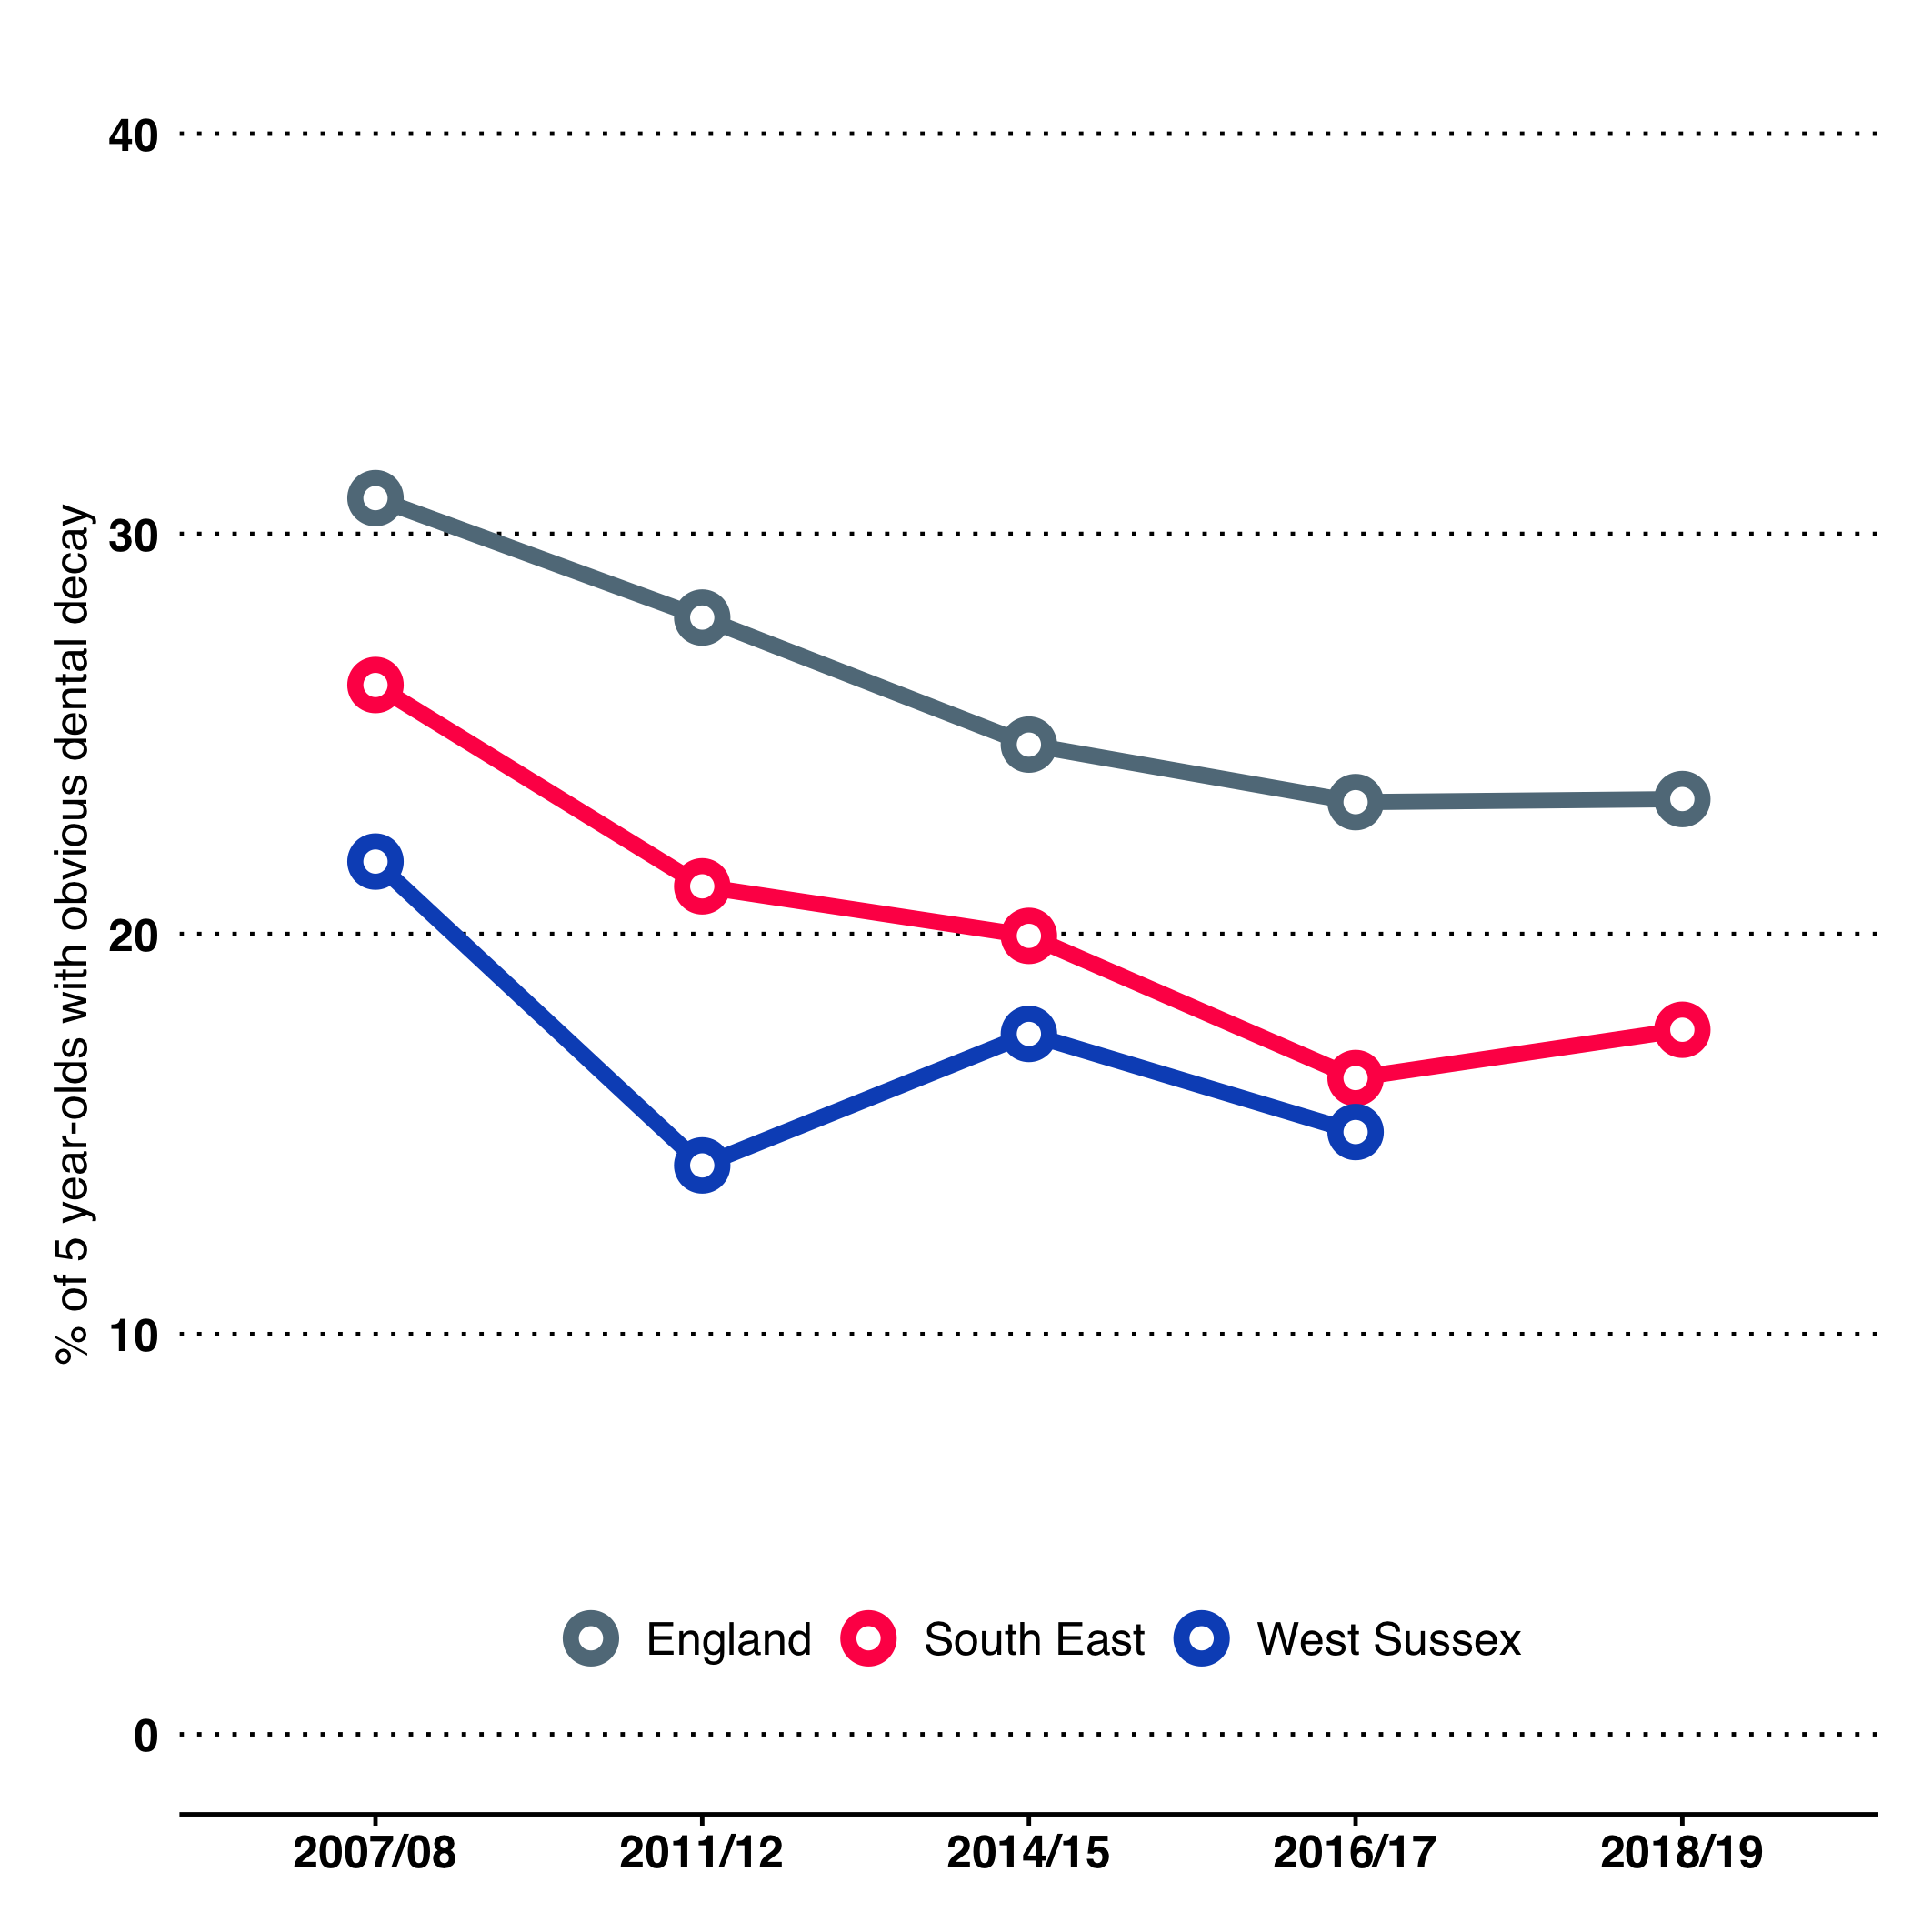
\includegraphics[width=\linewidth]{images/visual_dental_decay_5yos.png}
%	\label{fig:vodd_wsx}
%\end{figure}


%In 2016/17, dental services activity was greater overall than England, with the highest activity in Mid Sussex and the lowest in Chichester and Worthing.

%West Sussex children have a greater rate of "examinations" and "scale and polish" than nationally and lower rates of "permanent fillings and sealant restorations" in primary care, implying more check-ups help to prevent invasive treatments.

%Aside from using private dentistry, the most common reasons for not seeking a dental appointment in the last two years were residents not thinking they could get an NHS dentist and the belief they didn't need to see a dentist.

%\paragraph{Provision of dental services }
%In 2017/18, there were 146 dental contracts withinWest Sussex, covering general dentistry, community dental services and emergency access clinics. The required travelling distance is 10 miles or more for children living in some areas of Chichester district. 

%More children had seen a dentist (71\%, not including private dentists) than nationally in the 24 months prior to 2016/17. 

%Access rates were slightly better than England overall:
%\begin{itemize}
%    \item 6-12 year-olds had the highest rates, at 84.1\%
%    \item The 0-2 age group had the lowest rates, at 19.0\% vs. 21.7\% nationally. 
%\end{itemize}
 
%None of the districts in West Sussex fulfilled their NHS-contracted quota in 2016/17. Chichester, Arun, Mid Sussex and Worthing districts significantly underperformed.

%\subsubsection{Risk factors}
%More deprived local authorities have higher rates of dental decay (with the exception of Worthing), in line with the national pattern.

%Compared to England, West Sussex has a higher proportion of Special Educational Needs (SEN) children, who tend to have greater anxieties around seeing a dentist so are more at risk of poor oral health. Fewer SEN children had dental decay than nationally, although a higher percentage had substantial plaque compared to the South East region. 

%"Looked after" children are less likely to visit a dentist regularly and tend to have more dental disease and oral care neglect than those not in care. In West Sussex, a greater percentage of looked after children had seen the dentist than nationally (92.9\% vs. 84.4\%). 

\subsection{Health Related Behaviours and Healthy Weight}
\paragraph{Health-related behaviour of young people} 
Using the data from the 2014/15 national What About Youth (WAY) survey, 10.6\% of 15 year-olds in West Sussex stated that they were current smokers\footnote{The WAY survey data has been replaced by NHS Digital: Smoking, Drinking and Drug Use (SDD) in England as a PHOF indicator (previously 2.09i). However lack of local data in the SDD means the WAY survey remains the most recent estimate of smoking in young people in West Sussex.}. This is higher than England (8.2\%) and high amongst comparable authorities, although some caution is needed, given the lack of trend data and small sample sizes.

{\bfseries There were 195 hospital admissions for alcohol-specific conditions (of under 18s) in the period from 2018/19 to 2020/21. This is a rate of 36.9 per 100,000, which is significantly higher than the England rate of 29.3. These admissions have been increasing and are now at their highest level since 2011/12 to 2013/14, even as rates in England have fallen.}

The chlamydia detection rate \footnote{PHOF reference D02a.} remains below the England rate. In 2020, the rate was 1,003 per 100,000 15-24 year-olds and low compared with similar authorities.

West Sussex has a low teenage pregnancy rate\footnote{PHOF reference C02a.}, at 12.6 per 1,000 15-17 year-olds (179 conceptions) in 2019. This rate was slightly higher than in 2016 but remains low compared with England (rate of 15.7).

% Adur (rate of 14.8), Arun (18.9), Worthing (19.1) and Crawley (22.8) have rates similar to England.

{\bfseries The number of births to teenage mothers is less than a quarter of what it was ten years ago,} falling from 103 in 2010/2011 to 25 in 2020/21. 0.3\% of all births are to women in their teenage years. 

47.3\% of children aged 5-16 met the recommendations for physical activity in 2020/21\footnote{PHOF reference C10. The recommended physical activity is an average of at least 60 minutes moderate-vigorous intensity activity per day across the week.}, in line with England and national benchmark. The only lower tier authority in West Sussex with a sufficient sample size was Crawley, with 49.6\% of children which is also similar to the national figure.

\subsubsection{Healthy Weight - Reception and Year 6 Pupils}
In England in 2020/21, over a fifth of reception children were overweight or obese, increasing to over a third in Year 6. In West Sussex, the prevalence of obesity was lower than national levels, with 19.2\% of reception age children (4- 5 years old) and 28.8\% of Year 6 children (10-11 years old) measured as overweight or obese\footnote{PHOF references C09a and C09b.}.

% No lower tier data for 2020/21 at time of writing
% Within local authorities, the prevalence of overweight and obesity is varied. Arun, Worthing and Chichester had the highest prevalence of overweight and obesity among reception children (21.6\%, 21.5\% and 21.2\%, respectively) and Worthing had the highest prevalence among Year 6 children (32.3\%)

Inequalities in childhood obesity persist. For both school year groups, prevalence of excess weight among children living in the most deprived areas of West Sussex is greater than those living in the least deprived areas.

The Research Unit has drafted a briefing on data from the National Child Measurement Programme. This is available on the JSNA website.

\subsubsection{Education}
\paragraph{Early Years Provision, Education, NEET \& Progression to Higher Education}
Note: Unless stated, data for this section have been taken from the Department for Education Local authority interactive tool (LAIT). This is an interactive online tool. \url{https://www.gov.uk/government/publications/local-authority-interactive-tool-lait}

77\% of 2 year-olds in West Sussex benefited from funded early years (2 year-olds) in 2019. This is higher than the England rate and that of comparable authorities.

55\% of 2, 3 and 4 year-olds are in funded early provision with staff who have graduate status, similar to the England rate.

\paragraph{Special Educational Needs}

In January 2021 3.1\% of pupils attending a West Sussex school had a statement or Education, Health and Care (EHC) plan. This percentage is similar to regional and national percentages. The number of children on such plans has been increasing since 2018.

% There were 3,218 children with a moderate learning difficulty known to schools in 2018, and 348 with a severe learning disability.

As at 31 December 2021, 92.4\% of 16 and 17 year olds with SEN in West Sussex were in Education or Training. This is higher than both England and the average of the county's statistical neighbours.

\paragraph{16-17 year-olds not in education, employment or training (NEET)}

Compared to other authorities in the South East, West Sussex has the third highest proportion of 16-17 year-olds not in education, employment or training, at 7.7\% in 2020 (England 5.5\%, South East 6.4\%)\footnote{This is a West Sussex Plan priority. Refer the WSCC website for the latest data and commentary. The combined known and unknown status of NEET 16-17 year-olds is a PHOF indicator (B05).}. This represents 1320 young people in West Sussex.

Broken down, 5.5\% of this group has unknown status which, while lower than than in recent years is higher than both the average of statistical neighbours (3.4\%) and England (2.7\%). 

% (6.7\% of the total 16-17 year-old population). However, this portion of 16-17 year-olds has decreased, relative to 2016 figures, whilst the portion of NEET 16-17 year-olds with known status has increased (rising from 1.4\% to 2.4\% of the total 16-17 year-old population). 

\paragraph{School readiness} Overall, West Sussex compares poorly or similarly to the England level for school readiness measures\footnote{PHOF indicators B02a and B02b}, and performs significantly worse for children with free school meal status. West Sussex has been improving in recent years for these measures, however, and remains broadly comparable to statistical neighbours.

At Key Stage 2 (children aged 10-11 years), attainment is notably low, with 63\% of pupils achieving the expected standard in reading, writing and maths in 2019, and only 7\% of pupils attaining the higher standard (compared with 11\% nationally).

These figures have not been updated since the previous JSNA summary.

\begin{figure}[htp]
    \centering
    \caption{School readiness in West Sussex (2019)}
    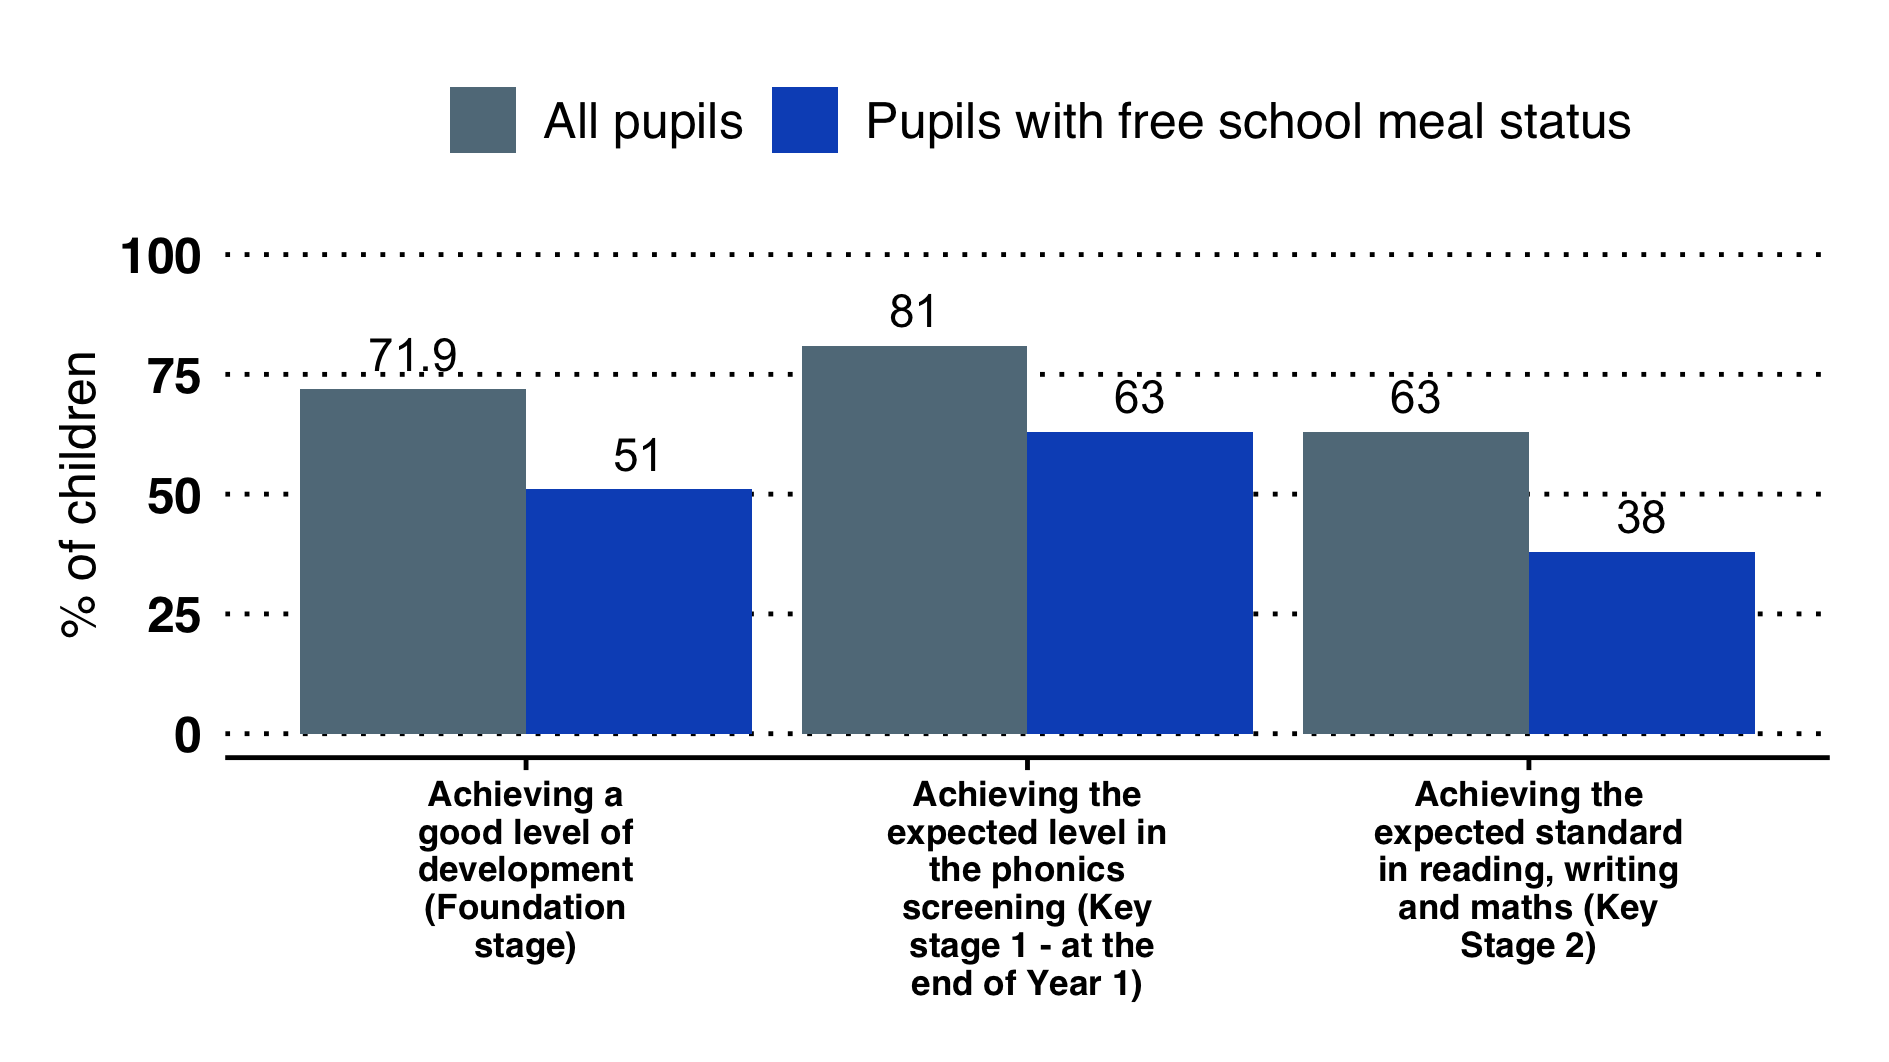
\includegraphics[width = \linewidth]{images/02_school_readiness_2019.png}
\end{figure}

At Key Stage 4 (GCSE level), attainment is above England overall (on the average P8 score measure) and in line with comparable authorities.

\paragraph{Progression to Higher Education (HE)} 40\% of all pupils progressed to higher education by age 19 in 2017/18, lower than England (43\%) and statistical neighbours (40.1\%). {\bfseries Significantly fewer pupils on free school meals progressed to HE, at 19\%} (England 27\%, statistical neighbours 16.5\%).

Data from the Office for Students shows some areas in West Sussex (including Littlehampton) are ranked in the lowest national quintile for progression to HE\footnote{Office for Students. POLAR - Participation of Local Areas. 2017.}.

\subsubsection{Social Care and Community Safety}
Note: Unless stated, data for this section have been taken from the Department for Education Local authority interactive tool (LAIT). This is an interactive online tool.\footnote{\url{https://www.gov.uk/government/publications/local-authority-interactive-tool-lait}}
\paragraph{Social Care and Criminal Justice}

As at 31 March 2021 there were 891 children looked after, a rate of 50 per 10,000. The rate in West Sussex remains lower than England, but similar to statistical neighbours. 80 children were unaccompanied asylum seeking children.

\paragraph{Outcomes for Children Looked After and Children Leaving Care}
In 2021, 8\% of care leavers were not in touch with the local authority. This was higher than England but similar to comparable local authorities. 31\% of children looked after are noted as "persistent absentees".

In relation to the emotional and mental wellbeing of children in care, in 2020/21, a higher percentage (50.6\%) of children in West Sussex were children with a 'cause for concern'\footnote{PHOF reference C12. Strengths and Difficulties Questionnaire (SDQ) scores come from the SDQ questionnaire, a survey required to be completed by for each child looked after aged 5 to 16 years. It has five sections (emotional difficulties; conduct problems; hyperactivity or inattention; friendships and peer groups; and positive behaviour) plus an "impact supplement" to assist in the prediction of emotional health problems. The questionnaire is completed by the child's main carer. A score of 0 to 13 is considered normal, 14 to 16 borderline, and 17 to 40 is a cause for concern.} (whereby they scored 17 or above on the Strengths and Difficulty questionnaire, which asks questions on a range of issues relating to emotional and mental wellbeing). This was significantly higher than England (36.8\%).

\paragraph{Criminal Justice}

First time entrants to the criminal justice system declined in the county, down to 74 per 1,000 10-17 year-olds in 2020, making the rate in West Sussex significantly lower than that of England (169.2) and the lowest in the South East (156.7).

\paragraph{Children in Need (CiN)} The Children in Need rate, as at 31 March 2021, was 330.0 per 10,000. This is lower than England but broadly in line with comparable authorities. As at March 2021, there were 5,853 children in need.

6.7\% of Children in Need had a recorded disability. This is much lower than the England rate of 12.7\%.

The rate (per 10,000) of referrals to social services increased year on year between 2014 and 2018, although it declined slightly in 2019 and 2020 to 516.0. This rate is similar to England but higher than comparable local authorities. In total there were 8,803 referrals.

Section 47 enquiries\footnote{This relates to enquiries where there is reasonable cause to suspect the child is suffering, or is likely to suffer significant harm. Local authorities carry out an assessment under section 47 of the Children Act 1989 to determine if steps are needed to safeguard the child. Where concerns are substantiated, and the child is judged to be at continuing risk, an initial child protection conference should be convened within 15 working days.} (started within year) remain fairly steady, at 188.8 per 10,000. This was higher than England and comparable authorities.

\paragraph{Children subject to a Child Protection Plan (CPP)} In 2021, the rate of children subject to a CPP was 53.8 per 10,000, higher than England and comparable authorities. The percentage of children who became subject to a CPP for a second or subsequent time held steady at approximately 25\%. This is higher than comparable authorities and England.

\subsubsection{Transition to Adult}
Some young people, including those in care and young people with health needs and disabilities, require additional support as they enter adulthood. Many young people will have on-going services and this can be a time of considerable anxiety.

National research shows disabled young people aged 16-24 are less satisfied with their lives than their peers. There is a tendency for support to fall away at key transition points as young people move from child to adult services.

Following transition from a residential school, young people may experience good access to frontline health and social services, but also very few opportunities to enter employment or further education; no additional improvements in communication, self-care or behaviours that challenge; a reduction in good support for behaviours that challenge and increased reliance on restrictive practices; limited access to specialist services; and living at distance from the family home.

% \subsubsection{Further information}
% This is a summary document. More detailed local analyses (alongside a whole host of national profiles!) are available, including the needs assessment and briefings highlighted below. If you have specific information requests please contact the team.

% Contacts in the West Sussex Public Health and Social Research Team for Starting Well:
% \begin{itemize}
%     \item Jacqueline Clay - jacqueline.clay@westsussex.gov.uk
%     \item Dr Verity Pinkney - verity. pinkney@westsussex.gov.uk
% \end{itemize} 